\section[Compute \texorpdfstring{$\pi$}{pi}]{Compute $\pi$}

\subsection{Buffon theorem}

Let's see an (inefficient) method to compute $\pi$:

\begin{theorem} (Buffon): If I throw randomly a needle of length 1 on a floor with planks of width 2, the probability of crossing a crack (i.e. overlap two planks) is $\frac{1}{\pi}$ (see figure \ref{needles}).
\end{theorem}


\begin{figure}[h]
\centering
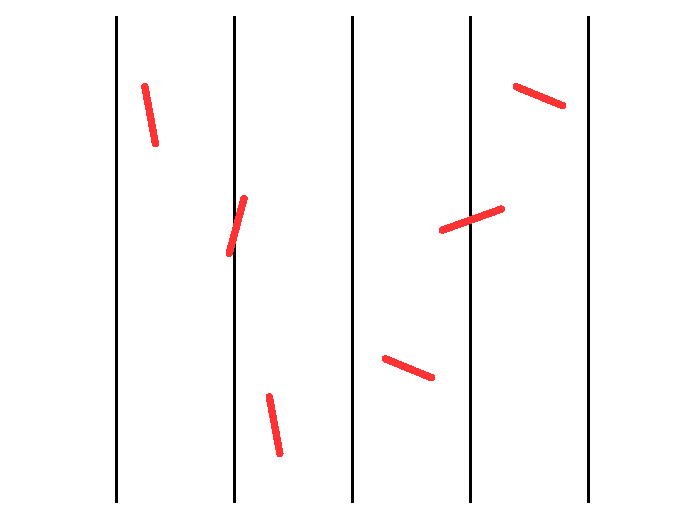
\includegraphics[scale=0.7]{images/needles.eps}
\caption{Needles of length 1 crossing cracks of width 2}
\label{needles}
\end{figure}

\paragraph*{Proof.}
\begin{enumerate}
\item Trigonometry + calculus: integrate over all angles and horizontal coordinates of needles.
\item Consider a needle of length $l$.
$E_l := $ expected number of cracks crossed by the needle $= \mathbb{E}(X_l)$, where $X_l$ is the number of cracks crossed. We have
$$
E_{2l} = \mathbb{E}(X_{2l}) = \mathbb{E}(X_l^1+X_l^2) = \mathbb{E}(X_l^1) + \mathbb{E}(X_l^2) = E_l + E_l = 2E_l
$$
More generally, $E_{l_1+l_2} = E_{l_1} + E_{l_2}$. So we see it follows a linear form: $E_l = \alpha l$, for some $\alpha$.\\
If $l=1$, as it never crosses twice, we can write 
$$
X_l = \left\{
      \begin{aligned}
        &1 \text{ if the needle crosses a crack}& \\
        &0 \text{ otherwise}& \\
      \end{aligned}
    \right.
$$
    So $E_l$ is the probability to cross a crack. Now we have to proof that $\alpha = \frac{1}{\pi}$.\\
Let be even more general: let's bend the needle. We have
$$
\mathbb{E}(\text{number of cracks crossed}) = E_{l_1} + E_{l_2}
= \alpha (l_1 + l_2)
= \alpha l
$$
with $l$ the total length of the needle. We can bend it several times...
$$
\mathbb{E}(\text{number of cracks crossed}) = \alpha \sum_i l_i = \alpha l
$$

\begin{figure}[h]
\centering
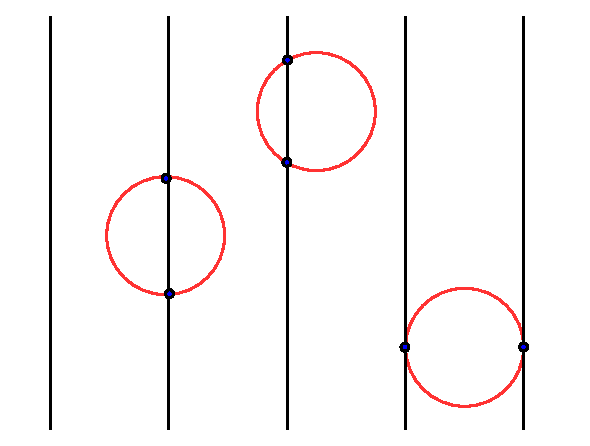
\includegraphics[scale=0.7]{images/circles.eps}
\caption{Circular needles of radius 1 crossing cracks of width 2}
\label{circles}
\end{figure}

In the limit, for a curved needle of length $l$, we always have $\mathbb{E}(\text{number of cracks crossed}) = \alpha l$. To fix $\alpha$, let's look at a circular needle of radius $1$, such that $E_l=2$, always (see figure \ref{circles})! We can write $E_{2\pi} = 2$, but $E_{2\pi} = \alpha 2 \pi$, and we conclude with $\alpha = \frac{1}{\pi} $.
\end{enumerate} 

We can then develop an algorithm to compute $\pi$:
\begin{itemize}
\item Throw a needle $n$ times on the floor (as in Buffon's theorem)
\item Count how many times a crack is crossed (define this number as $k$)
\item $\pi = \frac{n}{k}$
\end{itemize}

Accuracy of this algorithm? Let's look at its variance. Let
$$
X_i = \left\{
      \begin{aligned}
        &1 \text{ if the } i^{th} \text{ needle crosses a crack}& \\
        &0 \text{ otherwise}& \\
      \end{aligned}
    \right.
$$
As we have $\mathbb{E}(X_i)=\frac{1}{\pi}$ and $Var(X_i) = \frac{1}{\pi}(1-\frac{1}{\pi})$ and the $X_i$ are independant, it follows that
\begin{eqnarray*}
\mathbb{E}(\frac{\sum_i X_i}{n}) &=& \frac{1}{\pi} \\
Var(\frac{\sum_i X_i}{n}) &=& \frac{n \frac{1}{\pi}(1-\frac{1}{\pi})}{n^2} = \frac{1}{n}\frac{1}{\pi}(1-\frac{1}{\pi})
\end{eqnarray*}
We can now compute the standard deviation $\sigma = \frac{1}{\sqrt{n}}\sqrt{\frac{1}{\pi}(1-\frac{1}{\pi})}$ = typical error in $\frac{1}{\pi}$:
$$
\frac{k}{n} \in [\frac{1}{\pi}-\frac{2}{\sqrt{n}}\sqrt{\frac{1}{\pi}(1-\frac{1}{\pi})}; \frac{1}{\pi}+\frac{2}{\sqrt{n}}\sqrt{\frac{1}{\pi}(1-\frac{1}{\pi})}]
$$
with 95\% probability.\\
\textit{Remarks:}
\begin{itemize}
\item To gain one digit of accuracy, you need 100 times more throws: not good.
\item The result is possibly wrong, with some probability (here 5\%).
\end{itemize}